\documentclass[11pt,a4paper]{article}

% ---------------------------------------------------------------------------
% Abundant reactions in autocatalytic networks with locally ranked supplier
% cores.
%
% Author metadata: set the macros below before submission.  They are left
% blank deliberately.  \CompanionAuthor fills the author field of the
% companion-manuscript and repository citations in refs.bib.
% ---------------------------------------------------------------------------
\newcommand{\PaperAuthor}{}
\newcommand{\PaperAffiliation}{}
\newcommand{\PaperDate}{14 September 2026}
\newcommand{\CompanionAuthor}{Anonymous}

\usepackage[T1]{fontenc}
\usepackage[utf8]{inputenc}
\usepackage{lmodern}
\usepackage{microtype}
\usepackage[a4paper,margin=1.05in]{geometry}
\usepackage{amsmath,amssymb,amsthm,mathtools}
\usepackage{booktabs}
\usepackage{array}
\usepackage{enumitem}
\usepackage{xcolor}
\usepackage{graphicx}
\usepackage{tikz}
\usetikzlibrary{arrows.meta,positioning,calc,fit,backgrounds}
\usepackage{pgfplots}
\pgfplotsset{compat=1.18}
\renewcommand{\topfraction}{0.9}
\renewcommand{\textfraction}{0.05}
\renewcommand{\floatpagefraction}{0.75}
\usepackage[obeyspaces,spaces]{url}
\usepackage[numbers,sort&compress]{natbib}
\usepackage[colorlinks=true,linkcolor=blue!55!black,citecolor=blue!55!black,urlcolor=blue!55!black]{hyperref}
\hypersetup{pdftitle={Abundant reactions in autocatalytic networks with locally ranked supplier cores},
 pdfauthor={\PaperAuthor},
 pdfsubject={Half-frequency abundance for RAF families with a locally ranked complete-supplier core},
 pdfkeywords={autocatalytic sets, RAF theory, union-closed sets conjecture, Horn functions, dependency property, formal verification}}

\DeclareUrlCommand\lean{\urlstyle{tt}}
\setlist{itemsep=2pt,topsep=3pt}
\setlength{\emergencystretch}{1.5em}

\definecolor{substrate}{HTML}{245F91}
\definecolor{catalytic}{HTML}{B95112}
\definecolor{corefill}{HTML}{EDF4FA}
\definecolor{coreedge}{HTML}{9CBBD3}

\theoremstyle{plain}
\newtheorem{theorem}{Theorem}[section]
\newtheorem{proposition}[theorem]{Proposition}
\newtheorem{lemma}[theorem]{Lemma}
\newtheorem{corollary}[theorem]{Corollary}
\theoremstyle{definition}
\newtheorem{definition}[theorem]{Definition}
\newtheorem{example}[theorem]{Example}
\newtheorem{question}[theorem]{Question}
\theoremstyle{remark}
\newtheorem{remark}[theorem]{Remark}

\newcommand{\FF}{\mathcal F}
\newcommand{\BB}{\mathcal B}
\newcommand{\QQ}{\mathcal Q}
\newcommand{\N}{\mathbb N}
\newcommand{\R}{\mathbb R}
\newcommand{\E}{\mathbb E}
\newcommand{\after}{\mathrm{after}}
\DeclareMathOperator{\cat}{cat}

\title{Abundant reactions in autocatalytic networks\\ with locally ranked supplier cores}
\author{\PaperAuthor\\[2pt] {\small\itshape \PaperAffiliation}}
\date{\PaperDate}

\begin{document}
\maketitle

\begin{abstract}
A reflexively autocatalytic and food-generated set (RAF) of a catalytic reaction system is a set of reactions that can be built up from a food set and in which every reaction is catalysed from within. With the empty set adjoined, the RAFs of a finite system form a union-closed family, and Steel asked whether some reaction always lies in at least half of them. We prove this for every system containing a \emph{locally ranked complete-supplier core}: a nonempty set $U$ of reactions in which each reaction has one internal supplier producing all of its non-food reactants and, unless food already catalyses it, a catalyst, and in which the internal substrate-production digraph is acyclic. Nothing is assumed outside $U$: the surrounding system may contain arbitrary substrate cycles, alternative producers and catalytic feedback into the core, and the core itself need not be elementary. The proof identifies each exterior fibre of the RAF family exactly, through food closure of the combined selected set, with a supported family under an upward constraint, and applies the dependency counting injection of Lozin and Zamaraev. The resulting occupancy inequality holds in every exterior context and with the empty set counted, and it yields exterior-weighted and bounded-distortion sampling statements with the sharp constant $1/(1+\kappa)$, deterministic and expected bounds for the number of RAFs destroyed by deleting one core reaction, transport of the certificate across exterior edits, and distinct abundant reactions from disjoint cores. Every elementary core is a locally ranked supplier core, so the theorem strictly extends the elementary-core abundance theorem; a three-reaction system separates it from any hypothesis on the global substrate digraph. A uniform three-chain family with no elementary RAF shows that the core average is sharp while individual core reactions can be arbitrarily rare, and that the RAF family need not be the support family of any digraph. The main theorem and the source-level consequences are verified in Lean~4 against Mathlib.
\end{abstract}

\noindent\textbf{Keywords.} autocatalytic sets; RAF theory; union-closed sets conjecture; Horn functions; dependency property; formal verification.

\noindent\textbf{MSC 2020.} 05D05, 92C42, 06A15, 68V20.

\section{Introduction}\label{sec:intro}

\subsection{Autocatalytic sets and Steel's question}

Collectively autocatalytic sets were proposed by Kauffman~\cite{kauffman1986autocatalytic,kauffman1993origins} as a route by which a mixture of simple molecules could organise into a self-sustaining chemistry. Hordijk and Steel~\cite{hordijk2004detecting} made the idea precise in the RAF formalism. A \emph{catalytic reaction system} consists of molecule types, reactions with reactant and product sets, a distinguished \emph{food} set, and a catalysis relation. A set of reactions is \emph{food-generated} if all of its reactants can be produced from food, in some order, using only the selected reactions, and it is \emph{reflexively autocatalytic} if every selected reaction has a catalyst that is food or is produced by the selected reactions. A RAF is a nonempty set that is both. The largest RAF inside any given reaction set is computable in polynomial time, and the formalism has been developed extensively~\cite{steel2013minimal,hordijk2017chasing,steel2019autocatalytic,mossel2005random}.

The union of two RAFs is again a RAF. Adjoining the empty set, the RAFs of a finite system therefore form a \emph{union-closed family} of subsets of the reaction set, and the map sending an available reaction set to the largest RAF it contains is an interior operator. Steel~\cite{steel2023interior} studied this operator and asked, in his concluding section, whether there is always a reaction that lies in at least half the RAFs, for either an elementary or a general catalytic reaction system. A positive answer for all systems would follow from Frankl's union-closed sets conjecture~\cite{frankl1995extremal,bruhn2015journey}, which asserts that every finite union-closed family other than $\{\varnothing\}$ has an element lying in at least half of its members. That conjecture is open. After a long period in which only logarithmic bounds were known~\cite{wojcik1999union}, Gilmer~\cite{gilmer2022constant} proved a constant lower bound by an entropy argument, quickly improved to $(3-\sqrt5)/2\approx0.382$ and beyond~\cite{alweiss2022improved,chase2022approximate,sawin2022improved,cambie2022better}; the constant $1/2$ remains out of reach.

A companion paper~\cite{elementary2026} shows that the RAF version of the question has two faces. If the system contains an \emph{elementary core}, a nonempty RAF all of whose reactants are food, then a reaction of that core lies in at least half of all RAFs of the whole system, whatever the remaining reactions do. On the other hand, every finite union-closed family containing the empty set is the RAF family of a system without an elementary core, so a half-frequency theorem for the coreless class is equivalent to the unrestricted conjecture. The companion paper therefore asks which structural hypotheses on a system \emph{without} an elementary core imply abundance, and observes that such hypotheses must constrain reactant requirements, because the universal construction already makes the catalytic structure trivial.

This paper answers that question for a natural class. The elementary hypothesis says that core reactions need nothing but food. We replace it by two conditions on reactant supply \emph{inside the core only}: every core reaction has a single internal supplier providing all of its non-food reactants (and a catalyst, unless food already catalyses it), and the internal substrate-production digraph is acyclic. Both conditions are checked on the core incidences alone. Outside the core nothing is assumed.

\subsection{Main results}

Throughout, $\FF$ denotes the family of RAFs of a finite catalytic reaction system together with the empty set, $M=|\FF|$, $N=M-1$ is the number of nonempty RAFs, and $f(r)$ is the number of members of $\FF$ containing the reaction $r$. A reaction is \emph{abundant} if $2f(r)\ge M$. Because the empty set contributes to the denominator but to no numerator, abundance is slightly stronger than the half-frequency statement over nonempty RAFs alone; Steel's question is the weaker form, and all our positive results give the stronger one.

A reaction $p$ is a \emph{complete supplier} of a reaction $r$ if $p$ produces every non-food reactant of $r$ and, unless some food molecule catalyses $r$, some product of $p$ catalyses $r$. A nonempty set $U$ of reactions is a \emph{complete-supplier core} if every $r\in U$ has a complete supplier in $U$, and it is \emph{locally ranked} if there is a map $\lambda:U\to\N$ with $\lambda(p)<\lambda(r)$ whenever $p,r\in U$ and some product of $p$ is a non-food reactant of $r$ (Definition~\ref{def:core}). The rank condition inspects every internal substrate-production incidence, including self-incidences, not only the chosen suppliers; catalytic incidences are not part of it, and catalytic cycles inside the core are what typically make the core autocatalytic.

\begin{theorem}[Locally ranked supplier-core abundance; Theorem~\ref{thm:main}]\label{thm:intro-main}
Let $U$ be a locally ranked complete-supplier core of a finite catalytic reaction system. Then $U$ is a RAF, and some reaction of $U$ is abundant in $\FF$. More precisely, for every set $T$ of reactions outside $U$, the core parts $S=W\cap U$ of the members $W\in\FF$ with $W\setminus U=T$ have average size at least $|U|/2$, and consequently
\[
\sum_{W\in\FF}|W\cap U|\ \ge\ \tfrac12\,|U|\,M .
\]
\end{theorem}

The fibrewise form is the real content. The proof has two steps. The first (Lemma~\ref{lem:adapter}) is an exact description of each exterior fibre: for a fixed exterior selection $T$, a set $S\subseteq U$ satisfies $S\cup T\in\FF$ if and only if the exterior reactions of $T$ are supported in the food closure of $S\cup T$ and every selected core reaction has its non-food reactants and a catalyst produced by some selected reaction. The rank hypothesis is what turns these local producer requirements into genuine food generation; the exterior condition is evaluated through the actual closure of the combined set and is monotone in $S$, but nothing is assumed about $T$ on its own. The second step (Lemma~\ref{lem:count}) is the aggregate form of the counting theorem of Lozin and Zamaraev~\cite{lozin2024union} for Horn functions with a dependency property: a family of subsets of $U$ defined by an upward constraint together with per-element monotone support requirements, each of which is met whenever a designated companion is selected, has average member size at least $|U|/2$. The complete supplier is the companion. Summing over exterior fibres retains every exterior completion multiplicity and gives the global inequality, from which the witness follows by averaging.

The theorem strictly extends the elementary-core theorem of~\cite{elementary2026}: every elementary core is a locally ranked supplier core with constant rank (Proposition~\ref{prop:elementary}), while the three-reaction system of Section~\ref{sec:strict} has a locally ranked core that is not elementary, and its ambient substrate digraph has a cycle, so no hypothesis on the global substrate digraph covers it. The three-chain family of Section~\ref{sec:family} has no elementary RAF at all.

The fibrewise inequality has consequences that a bare existence statement would not give (Section~\ref{sec:consequences}).
\begin{itemize}
\item \emph{Transport and disjoint witnesses.} The hypotheses inspect only the core incidences, the food set and the catalysis relation, so the conclusion survives arbitrary edits of exterior reactions, enlargement of food and addition of catalytic incidences (Corollary~\ref{cor:transport}). Pairwise disjoint cores give distinct abundant reactions.
\item \emph{Weighting.} The half bound survives any nonnegative reweighting of exterior contexts (Corollary~\ref{cor:weights}). If instead each member of $\FF$ receives a weight that varies by a factor at most $\kappa$ within every exterior fibre, the expected core occupancy is at least $|U|/(1+\kappa)$ and some core reaction has weighted frequency at least $1/(1+\kappa)$; the constant is sharp (Theorem~\ref{thm:distortion}).
\item \emph{Deletion.} Some core reaction, when deleted, destroys at least half of the nonempty RAFs, leaving at most $\lfloor(N-1)/2\rfloor$; a uniformly random core reaction leaves at most $(N-1)/2$ in expectation (Proposition~\ref{prop:delete}).
\end{itemize}

Section~\ref{sec:examples} gives the examples and sharpness statements. A uniform family with three chains of length $\ell$ and three gates (Section~\ref{sec:family}) has exactly $\ell+8$ members in $\FF$, its designated core $B$ has average occupancy exactly one half, and yet its individual core reactions have frequencies ranging from $(\ell+4)/(\ell+8)\to1$ down to $4/(\ell+8)\to0$: the certificate identifies a set containing a witness, not the witness. The family has no elementary RAF, has transversal number three, has exactly three irreducible RAFs whose unions do not exhaust $\FF$, and is not the support family of any directed graph on its reactions, so the digraph-support characterisation of~\cite{digraph2026} does not apply to it. It admits a conservation bookkeeping that leaves $\FF$ unchanged (Proposition~\ref{prop:waste}). Section~\ref{sec:algorithms} separates candidate validation, which is quadratic in the core and needs no enumeration, from discovery and from witness identification. Section~\ref{sec:scope} lists what is not claimed and the open questions this leaves.

\subsection{Relation to prior work and what is new}

The RAF framework and the question are due to Hordijk and Steel~\cite{hordijk2004detecting} and Steel~\cite{steel2023interior}. The counting kernel is Theorem~4 of Lozin and Zamaraev~\cite{lozin2024union}, which proves Frankl's conjecture for Boolean functions admitting a Horn DNF in which every variable occurring negatively has a companion occurring positively in each term where it is negative. The elementary-core theorem, its fibrewise form and its exterior-weighted, cycle and disjoint-core consequences are proved in the companion paper~\cite{elementary2026}; that paper also introduced the exterior-conditioned application of the counting injection. What is new here is (i) the localisation of the hypothesis to reactant supply inside a designated core, which admits non-food reactants in the core and arbitrary substrate cycles outside it; (ii) the exact closure-conditioned fibre representation through the combined selected set, which is what makes the localisation sound, together with the rank induction that establishes food generation; (iii) the bounded-distortion sampling theorem with its sharp constant; (iv) the deletion bounds; and (v) the uniform three-chain family, with its exact frequencies, its structural properties and its conservation lift. An earlier version of the theorem required a rank on the substrate digraph of the whole system; the three-reaction example of Section~\ref{sec:strict} shows that the local version is strictly stronger, and both versions are compiled. We make no claim on the unrestricted conjecture, on systems with three non-food-ready reactions in general, or on the kinetics of RAF operation.

The classical observation that a union-closed family containing a singleton or a two-element set satisfies the conjecture is due to Sarvate and Renaud~\cite{sarvate1989union} (see also Poonen~\cite{poonen1992union}). Reimer's average set size theorem~\cite{reimer2003average} gives average member size at least $\frac12\log_2N$ for any union-closed family; our occupancy inequalities are of the same average-size type but give the bound $|U|/2$ under the structural hypothesis, for the core coordinates, and in every exterior fibre separately.

\subsection{Formal verification}

The main theorem and the source-level consequences marked in Appendix~\ref{app:lean} have been formalised in Lean~4~\cite{demoura2021lean} against Mathlib~\cite{mathlib2020} directly from the literal RAF semantics of Section~\ref{sec:prelim}, compiled with warnings as errors, and depend only on the standard axioms \lean{Classical.choice}, \lean{Quot.sound} and \lean{propext}. The formal main theorem takes an arbitrary system, a core, a rank and the supplier data as inputs and returns RAF status, the fibre inequalities, the global inequality and the witness; the desired average is not an input. The paper is written to be read without the formal development; the appendix states exactly which forms were compiled and which statements (the parametric family, the conservation lift, the general exterior-edit transport and the deletion interpretation) are ordinary mathematics only.

\section{Ordinary RAF semantics and the source criterion}\label{sec:prelim}

\begin{definition}[Catalytic reaction system]\label{def:crs}
A finite catalytic reaction system $\QQ$ consists of a finite molecule set $X$, a finite reaction set $R$, a food set $F\subseteq X$, reactant and product sets $\rho(r),\pi(r)\subseteq X$ for each $r\in R$, and catalyst sets $C(r)\subseteq X$. Distinct reactions are distinct even if their incidence data coincide. For $W\subseteq R$ the \emph{food closure} is
\[
 H_0(W)=F,\qquad
 H_{j+1}(W)=H_j(W)\cup\bigcup_{r\in W,\ \rho(r)\subseteq H_j(W)}\pi(r),
 \qquad H(W)=\bigcup_{j\ge0}H_j(W).
\]
Catalysis plays no role in this iteration. A nonempty $W\subseteq R$ is a \emph{RAF} if for every $r\in W$,
\[
 \rho(r)\subseteq H(W)\qquad\text{and}\qquad C(r)\cap H(W)\ne\varnothing .
\]
\end{definition}

The first condition is food generation, the second is reflexive autocatalysis evaluated in the closure of the selected set. Write
\begin{equation}\label{eq:family}
 \FF=\{\varnothing\}\cup\{W\subseteq R:\ W\text{ is a RAF}\},\quad
 M=|\FF|,\quad N=M-1,\quad f(r)=|\{W\in\FF:\ r\in W\}| .
\end{equation}
A reaction is \emph{abundant} if $2f(r)\ge M$. A reaction is \emph{food-ready} if $\rho(r)\subseteq F$, and an \emph{elementary core} is a nonempty RAF consisting of food-ready reactions~\cite{elementary2026}. Since a union of RAFs is a RAF, $\FF$ is union-closed, and an abundant reaction is exactly a witness for Frankl's conjecture in $\FF$.

\begin{definition}[Complete suppliers, cores and local rank]\label{def:core}
A reaction $p$ is a \emph{complete supplier} of a reaction $r$ if
\begin{equation}\label{eq:supplier}
 \rho(r)\setminus F\subseteq\pi(p)\qquad\text{and}\qquad
 \bigl(C(r)\cap F\ne\varnothing\ \text{ or }\ C(r)\cap\pi(p)\ne\varnothing\bigr).
\end{equation}
A nonempty set $U\subseteq R$ is a \emph{complete-supplier core} if for each $r\in U$ there is $d(r)\in U$ that is a complete supplier of $r$. It is \emph{locally ranked} if there is a map $\lambda:U\to\N$ such that
\begin{equation}\label{eq:rank}
 p,r\in U,\quad \pi(p)\cap(\rho(r)\setminus F)\ne\varnothing
 \quad\Longrightarrow\quad\lambda(p)<\lambda(r).
\end{equation}
A \emph{certificate} for $U$ is a choice of $\lambda$ and of the supplier map $d$.
\end{definition}

Condition~\eqref{eq:rank} says that the \emph{internal substrate-production digraph} of $U$, with an edge $p\to r$ whenever some product of $p$ is a non-food reactant of $r$, is acyclic; self-loops are excluded in particular. It inspects every internal producer alternative, not only the chosen suppliers. Catalytic incidences do not define its edges, and catalytic cycles inside $U$ are allowed and typical. The supplier condition is an existence condition: other producers and other catalysts of $r$, inside or outside $U$, remain allowed. Nothing whatever is required of the reactions outside $U$.

\begin{proposition}[Elementary cores are locally ranked supplier cores]\label{prop:elementary}
Every elementary core is a locally ranked complete-supplier core, with constant rank.
\end{proposition}
\begin{proof}
Let $U$ be a nonempty RAF of food-ready reactions. Since every $r\in U$ has $\rho(r)\setminus F=\varnothing$, the reactant clause of~\eqref{eq:supplier} holds for any $p$, and there are no internal substrate-production incidences, so~\eqref{eq:rank} holds for $\lambda\equiv0$. For the catalyst clause, $U$ is a RAF, so $C(r)\cap H(U)\ne\varnothing$. Every molecule of $H(U)$ is food or a product of some reaction of $U$, because the closure iteration only adds products of selected reactions. Hence either food catalyses $r$ or some $p\in U$ has $C(r)\cap\pi(p)\ne\varnothing$; in the first case take $d(r)=r$, in the second $d(r)=p$.
\end{proof}

The converse fails: the core of Section~\ref{sec:strict} contains a reaction with a non-food reactant, and the family of Section~\ref{sec:family} has no elementary RAF.

\begin{remark}[What the hypothesis excludes]\label{rem:excludes}
Two features of Definition~\ref{def:core} are forced. First, the rank condition cannot be dropped. With $F=\{f\}$ and two reactions $p:y\to x$ and $q:x\to y$, both catalysed by $f$, each is a complete supplier of the other, but no nonempty set is food-generated, so $\FF=\{\varnothing\}$ and there is no RAF at all. The supplier condition alone describes support relations that are consistent but never seeded. Second, the single-supplier condition cannot be weakened to independent suppliers of different reactants. The universal producer--gate construction of~\cite{elementary2026}, which realises every union-closed family, has an acyclic substrate digraph, one catalyst per reaction and one food molecule; its gates need marker molecules from several different producers, and the producer that supplies a gate's catalyst supplies none of its markers. No single reaction meets every requirement of a gate, and this is precisely where the counting injection of Section~\ref{sec:count} loses the common coordinate that prevents collisions. Any sufficient condition satisfied by that construction would settle the unrestricted conjecture.
\end{remark}

\begin{theorem}[Locally ranked supplier-core abundance]\label{thm:main}
Let $U$ be a locally ranked complete-supplier core of a finite catalytic reaction system. Then $U$ is a RAF. For every $T\subseteq R\setminus U$ let
\begin{equation}\label{eq:fibredef}
 \BB_T=\{S\subseteq U:\ S\cup T\in\FF\}
\end{equation}
be the exterior fibre over $T$. Then
\begin{align}
 |U|\,|\BB_T|&\le2\sum_{S\in\BB_T}|S|\qquad\text{for every }T\subseteq R\setminus U,\label{eq:fibre}\\
 |U|\,M&\le2\sum_{W\in\FF}|W\cap U|,\label{eq:global}\\
 \exists\,r\in U:\quad M&\le2f(r).\label{eq:witness}
\end{align}
No restriction is placed on the substrate or supplier structure outside $U$.
\end{theorem}

Inequality~\eqref{eq:fibre} is trivially true when $\BB_T$ is empty, and it says that in a nonempty fibre the average core occupancy is at least $|U|/2$. The empty fibre $T=\varnothing$ contains $\varnothing$ and $U$ itself.

\section{Proof of the main theorem}\label{sec:proof}

\subsection{The exact closure adapter}\label{sec:adapter}

For a reaction $r$ and a set $W\subseteq R$, let $L_r(W)$ denote the conjunction
\begin{equation}\label{eq:local}
 \forall x\in\rho(r)\setminus F\ \ \exists p\in W:\ x\in\pi(p),
 \qquad\text{and}\qquad
 C(r)\cap F\ne\varnothing\ \ \text{or}\ \ \exists p\in W:\ C(r)\cap\pi(p)\ne\varnothing .
\end{equation}
This is the \emph{local support predicate}: every non-food reactant of $r$ has a selected producer, and $r$ has a food catalyst or a selected producer of a catalyst. It is monotone in $W$. It looks only at products of selected reactions and not at whether those reactions are themselves enabled; that is the gap that the rank hypothesis will close. A complete supplier of $r$ meets every clause of $L_r$ at once:
\begin{equation}\label{eq:supplier-local}
 d(r)\in W\quad\Longrightarrow\quad L_r(W).
\end{equation}

Fix $T\subseteq R\setminus U$ and define the \emph{exterior predicate} on subsets $S\subseteq U$ by
\begin{equation}\label{eq:exterior}
 K_T(S)\quad\Longleftrightarrow\quad
 \forall t\in T:\ \ \rho(t)\subseteq H(S\cup T)\ \text{ and }\ C(t)\cap H(S\cup T)\ne\varnothing .
\end{equation}
Food closure is monotone under addition of selected reactions, so $K_T$ is upward in $S$. It is evaluated through the closure of the combined set $S\cup T$; nothing is asserted about $T$ in isolation, and the example of Section~\ref{sec:strict} shows that $T$ need not be food-generated on its own.

\begin{lemma}[Exact fibre membership]\label{lem:adapter}
Let $U$ satisfy the rank condition~\eqref{eq:rank}, let $T\subseteq R\setminus U$, and let $S\subseteq U$. Then
\begin{equation}\label{eq:adapter}
 S\cup T\in\FF\quad\Longleftrightarrow\quad K_T(S)\ \text{ and }\ \forall r\in S:\ L_r(S\cup T).
\end{equation}
\end{lemma}
\begin{proof}
Write $W=S\cup T$. If $W=\varnothing$ both sides hold vacuously. Suppose $W$ is a nonempty RAF. The exterior clauses of $K_T(S)$ are the RAF conditions for the reactions of $T$. For $r\in S$, every non-food reactant $x$ of $r$ lies in $H(W)$, and every molecule of $H(W)$ is food or a product of a reaction of $W$, so $x$ has a selected producer; likewise a catalyst of $r$ in $H(W)$ is food or a product of a selected reaction. Hence $L_r(W)$.

Conversely assume the right-hand side and $W\ne\varnothing$. First, every product of a reaction $t\in T$ lies in $H(W)$: the reactants of $t$ lie in $H(W)$ by $K_T(S)$, there are finitely many of them, so they all lie in some stage $H_j(W)$, and then $\pi(t)\subseteq H_{j+1}(W)$. Next we show by strong induction on $\lambda(r)$ that every $r\in S$ has $\rho(r)\subseteq H(W)$. Let $x\in\rho(r)\setminus F$. By $L_r(W)$ there is $p\in W$ with $x\in\pi(p)$. If $p\in T$ then $x\in H(W)$ by the first step. If $p\in S$ then $x\in\pi(p)\cap(\rho(r)\setminus F)$, so~\eqref{eq:rank} gives $\lambda(p)<\lambda(r)$; by induction $\rho(p)\subseteq H(W)$, so $p$ is enabled at some finite stage and $x\in\pi(p)\subseteq H(W)$. Food reactants are in $H_0(W)$. Thus $W$ is food-generated, and every product of every reaction of $W$ lies in $H(W)$. Now the catalyst clause of $L_r(W)$ for $r\in S$ gives a catalyst of $r$ that is food or a product of a selected reaction, hence lies in $H(W)$; and the catalyst clauses for $t\in T$ are part of $K_T(S)$. So $W$ is a RAF.

The induction can be made explicit in closure stages: let $J$ be a stage by which the reactants of every $t\in T$ are available, so that $\pi(t)\subseteq H_{J+1}(W)$; then the reactants of a selected core reaction of rank $n$ lie in $H_{J+n+1}(W)$. This is the form used in the formal proof.
\end{proof}

The rank is used only inside $S$: exterior producers are handled by actual closure, whatever their own structure, and the induction descends through core producers only. This is why no acyclicity is needed outside $U$.

\subsection{The common-dependency counting argument}\label{sec:count}

The counting statement below is the aggregate form of Theorem~4 of Lozin and Zamaraev~\cite{lozin2024union}, who proved Frankl's conjecture for the families defined by Horn functions with their dependency property. In the present formulation the members of the family are the sets $S$ satisfying an upward constraint $K$ together with, for every selected element $r$, a monotone support requirement $L_r$; the dependency property is that each $L_r$ is met whenever a designated companion $d(r)$ is selected. An upward constraint corresponds to terms without a negative literal, which satisfy the dependency property vacuously, and grouping all Horn terms with the same head into one monotone predicate changes nothing in the injection. We include the proof because the paper is meant to be self-contained and because the formalisation follows it literally. The companion paper~\cite{elementary2026} uses the same lemma.

\begin{lemma}[Conditioned occupancy]\label{lem:count}
Let $U$ be a finite set, let $K$ and $L_r$ ($r\in U$) be upward predicates on subsets of $U$, and let $d:U\to U$ satisfy $d(r)\in S\Rightarrow L_r(S)$ for all $r$ and $S$. Put
\[
 \BB=\{S\subseteq U:\ K(S)\ \text{and}\ \forall r\in S,\ L_r(S)\}.
\]
Then $|U|\,|\BB|\le2\sum_{S\in\BB}|S|$.
\end{lemma}
\begin{proof}
Work with deletion sets $D=U\setminus S$ and define
\[
 P(D)=\neg K(U\setminus D),\qquad B_r(D)=\neg L_r(U\setminus D).
\]
Both are upward in $D$, and $B_r(D)$ implies $d(r)\in D$ (otherwise $d(r)\in U\setminus D$ would force $L_r$). Call $D$ \emph{bad} if $P(D)$ holds or some $r\notin D$ has $B_r(D)$; the bad sets are exactly the complements of the sets outside $\BB$. A \emph{cell} is a pair $(D,a)$ with $D$ bad and $a\in U$; it is a \emph{zero cell} if $a\notin D$ and a \emph{one cell} if $a\in D$. We construct an injection from zero cells to one cells.

Let $(D,a)$ be a zero cell. If $P(D)$ holds, or some $q\ne a$ with $q\notin D$ has $B_q(D)$, map it \emph{horizontally} to $(D\cup\{a\},a)$; by upwardness $P$ or $B_q$ persists, and $q\notin D\cup\{a\}$, so the image row is bad, and it is a one cell. Otherwise $P(D)$ fails and $a$ is the unique element outside $D$ whose requirement fails, so $B_a(D)$ holds; map \emph{vertically} to $(D,d(a))$, which is a one cell because $B_a(D)\Rightarrow d(a)\in D$.

Two horizontal images coincide only if their marks coincide and their rows, obtained by removing the mark, coincide. Two vertical images coincide only if their rows coincide, and then their marks are the unique failing elements of that row, hence coincide. Suppose finally that a horizontal image $(D\cup\{a\},a)$ equals a vertical image $(D',d(b))$ of a zero cell $(D',b)$. Then $D'=D\cup\{a\}$ and $a=d(b)$, and by verticality $P(D')$ fails while $b$ is the unique failing element outside $D'$. Since $(D,a)$ went horizontally, either $P(D)$ holds, which would persist to $D'$, or some $q\ne a$ with $q\notin D$ has $B_q(D)$; then $q\notin D'$ and $B_q(D')$, so $q=b$. But $B_b(D)$ forces $d(b)=a\in D$, contradicting $a\notin D$. Hence the map is injective.

Over the full Boolean cube $2^U$ there are as many zero cells as one cells, by complementation. The bad rows contribute at most as many zero cells as one cells, so the remaining rows, the complements of the members of $\BB$, contribute at least as many zero cells as one cells: $\sum_{S\in\BB}|S|\ge\sum_{S\in\BB}(|U|-|S|)$, which is the claim. It holds trivially if $\BB$ is empty.
\end{proof}

\subsection{Exact aggregation}\label{sec:aggregate}

\begin{proof}[Proof of Theorem~\ref{thm:main}]
Fix $T\subseteq R\setminus U$. Apply Lemma~\ref{lem:count} to the ground set $U$, the upward exterior predicate $K_T$ of~\eqref{eq:exterior}, and the internal predicates $S\mapsto L_r(S\cup T)$, which are upward in $S$ and satisfy the dependency condition by~\eqref{eq:supplier-local}. Lemma~\ref{lem:adapter} identifies the family $\BB$ of the counting lemma with the fibre $\BB_T$ of~\eqref{eq:fibredef}, which proves~\eqref{eq:fibre}.

For $T=\varnothing$ and $S=U$ the exterior predicate is vacuous and every internal predicate holds by~\eqref{eq:supplier-local}, so Lemma~\ref{lem:adapter} and $U\ne\varnothing$ show that $U$ is a RAF.

Every $W\in\FF$ decomposes uniquely as $W=(W\cap U)\cup(W\setminus U)$ with $W\cap U\in\BB_{W\setminus U}$, so $\FF$ is the disjoint union over $T$ of the sets $\{S\cup T:S\in\BB_T\}$, with $|\{S\cup T:S\in\BB_T\}|=|\BB_T|$. Summing~\eqref{eq:fibre} over $T$ gives~\eqref{eq:global} with no change of measure. Finally $\sum_{W\in\FF}|W\cap U|=\sum_{r\in U}f(r)$; if $2f(r)<M$ for every $r\in U$, summing the strict inequalities contradicts~\eqref{eq:global}. This proves~\eqref{eq:witness}.
\end{proof}

\begin{remark}
The proof never assumes that the exterior selection $T$ is a RAF, that it is food-generated on its own, or that $U$ is the largest RAF. It retains each original reaction subset and each exterior completion multiplicity: fibres with many completions weigh more in~\eqref{eq:global}, exactly as they do in $f(r)$. Replacing the exterior by a separately food-generated subsystem, a feasible trace with uniform weight, or a list of irreducible RAFs would change the measure and break the identity $\sum_W|W\cap U|=\sum_{r\in U}f(r)$.
\end{remark}

\section{Consequences}\label{sec:consequences}

\subsection{Transport across exterior edits and distinct witnesses}

\begin{corollary}[Transport and disjoint cores]\label{cor:transport}
Let $U$ be a locally ranked complete-supplier core of $\QQ$ with certificate $(\lambda,d)$.
\begin{enumerate}[label=(\alph*)]
\item If $\QQ'$ is obtained from $\QQ$ by adding, deleting or editing reactions outside $U$, by enlarging the food set, and by adding catalytic incidences, while the reactant and product sets of the reactions of $U$ are unchanged, then $(\lambda,d)$ certifies $U$ in $\QQ'$; hence $U$ is a RAF of $\QQ'$ and contains a reaction abundant in $\FF(\QQ')$.
\item If $U_1,\dots,U_k$ are pairwise disjoint locally ranked complete-supplier cores of $\QQ$, then $\QQ$ has $k$ distinct abundant reactions $r_i\in U_i$.
\end{enumerate}
\end{corollary}
\begin{proof}
(a) Conditions~\eqref{eq:supplier} and~\eqref{eq:rank} mention only $F$, the incidences of reactions in $U$ and the catalysis relation. Enlarging $F$ shrinks each $\rho(r)\setminus F$, which can only remove reactant requirements and internal substrate incidences; enlarging the catalysis relation can only add catalyst options; exterior edits change nothing that is inspected. So the certificate remains valid and Theorem~\ref{thm:main} applies to $\QQ'$. (b) Choose an abundant $r_i\in U_i$ by Theorem~\ref{thm:main}; disjointness makes the choices distinct. No independence between the cores is needed.
\end{proof}

The witness in (a) may change with the surrounding system: the companion paper gives an elementary core $\{a,b\}$ whose abundant reaction is $a$ in one exterior and $b$ in another~\cite[Example~5.2]{elementary2026}. No single reaction is asserted to work for all embeddings.

\subsection{Exterior weighting and bounded distortion}

\begin{corollary}[Exterior weights]\label{cor:weights}
Let $h:2^{R\setminus U}\to[0,\infty)$ and suppose $Z=\sum_{W\in\FF}h(W\setminus U)>0$. Put $\mu(W)=h(W\setminus U)/Z$. Then $\E_\mu|W\cap U|\ge|U|/2$, and some $r\in U$ satisfies $\mu(r\in W)\ge1/2$.
\end{corollary}
\begin{proof}
Multiply~\eqref{eq:fibre} by $h(T)$, sum over $T$, reindex by $W=S\cup T$ and divide by $Z$. The identity $|W\cap U|=\sum_{r\in U}\mathbf1_{\{r\in W\}}$ gives the witness by averaging over $U$.
\end{proof}

Indicator weights condition on any collection of exterior contexts, including a single fibre. Within a fibre all compatible core subsets receive equal weight. The next statement relaxes this.

\begin{theorem}[Bounded within-fibre distortion]\label{thm:distortion}
Let $\kappa\ge1$ and let $w:\FF\to[0,\infty)$ have positive total mass $Z$. Suppose that for every $T\subseteq R\setminus U$ there is $b_T\ge0$ with
\begin{equation}\label{eq:distortion-hyp}
 b_T\le w(S\cup T)\le\kappa\,b_T\qquad\text{for all }S\in\BB_T .
\end{equation}
Then for $\mu=w/Z$,
\begin{equation}\label{eq:distortion}
 \E_\mu|W\cap U|\ \ge\ \frac{|U|}{1+\kappa},\qquad
 \exists\,r\in U:\ \ \mu(r\in W)\ \ge\ \frac1{1+\kappa}.
\end{equation}
The constant $1/(1+\kappa)$ is sharp for every $\kappa\ge1$. In particular~\eqref{eq:distortion} applies to weights $w(S\cup T)=h(T)\,a_T(S)$ whenever the positive within-fibre factors $a_T$ have maximum-to-minimum ratio at most $\kappa$.
\end{theorem}
\begin{proof}
Fix $T$ with $b_T>0$; fibres with $b_T=0$ carry no mass. Let $n=|U|$, write $X(S)=|S|/n\in[0,1]$, and let $\E_T$ denote uniform expectation over $\BB_T$, so that $\E_TX\ge1/2$ by~\eqref{eq:fibre}. Put $a(S)=w(S\cup T)/b_T\in[1,\kappa]$, $A=\E_T[aX]$ and $B=\E_T[a(1-X)]$. Then
\[
 A\ge\E_TX,\qquad B\le\kappa\,\E_T[1-X]=\kappa(1-\E_TX)\le\kappa\,\E_TX\le\kappa A,
\]
so $A/(A+B)\ge1/(1+\kappa)$. Since $A/(A+B)=\sum_{S\in\BB_T}w(S\cup T)|S|\,/\,\bigl(n\sum_{S\in\BB_T}w(S\cup T)\bigr)$, this says $\sum_{S\in\BB_T}w(S\cup T)|S|\ge\frac n{1+\kappa}\sum_{S\in\BB_T}w(S\cup T)$. Summing over $T$ and dividing by $Z$ gives the first inequality of~\eqref{eq:distortion}; the coordinate identity gives the witness. For sharpness take $\FF=\{\varnothing,U\}$ (for instance the all-or-none module of Example~\ref{ex:modules} with $k=1$), which is a single fibre, with $w(\varnothing)=\kappa$ and $w(U)=1$: then $\E_\mu|W\cap U|=|U|/(1+\kappa)$ and every $r\in U$ has $\mu(r\in W)=1/(1+\kappa)$.
\end{proof}

These are structural sampling statements about the set family $\FF$. A kinetic interpretation would require an independent derivation of the sampling weights and of the distortion bound, and each chosen weighting has its own witness.

\subsection{Reaction deletion}

Deleting a reaction $r$ from $\QQ$ means removing it from $R$ while retaining the food set and the incidence data of all other reactions.

\begin{proposition}[Deletion bounds]\label{prop:delete}
Let $U$ be a locally ranked complete-supplier core and let $N$ be the number of nonempty RAFs of $\QQ$. For any reaction $r$, the nonempty RAFs of $\QQ$ with $r$ deleted are exactly the nonempty RAFs of $\QQ$ not containing $r$, so their number is $N_\after(r)=N-f(r)$. Consequently there is $r\in U$ with
\begin{equation}\label{eq:delete}
 N_\after(r)\ \le\ \Bigl\lfloor\frac{N-1}2\Bigr\rfloor ,
\end{equation}
and if $r$ is chosen uniformly at random from $U$ then
\begin{equation}\label{eq:expecteddelete}
 \E\,N_\after(r)\;=\;N-\frac1{|U|}\sum_{r\in U}f(r)\ \le\ \frac{N-1}2 .
\end{equation}
\end{proposition}
\begin{proof}
For $W\subseteq R\setminus\{r\}$, the closure iteration of Definition~\ref{def:crs} uses only the reactions of $W$ and their incidence data, which are the same before and after the deletion; so $H(W)$, and hence the RAF status of $W$, is unchanged. Thus the surviving RAFs are the original RAFs omitting $r$, and $N_\after(r)=N-f(r)$. By~\eqref{eq:witness} some $r\in U$ has $2f(r)\ge M=N+1$, so $f(r)\ge\lceil(N+1)/2\rceil$ and $N-f(r)\le\lfloor(N-1)/2\rfloor$. Averaging the identity over $U$ and applying~\eqref{eq:global} gives~\eqref{eq:expecteddelete}.
\end{proof}

The deterministic bound identifies a set containing a successful deletion; the expectation bound requires no individual frequencies. Both concern the \emph{number of RAF organisations}, not viability, a specified product, flux or persistence. Repeated halving requires a fresh certificate after each deletion, since deleting a core reaction destroys the core. Section~\ref{sec:twelve} shows that individual core deletions can perform much worse than the expectation.

\section{Examples and sharpness}\label{sec:examples}

\subsection{A strict extension beyond global substrate rank}\label{sec:strict}

\begin{example}\label{ex:strict}
Let $F=\{f\}$ and take three reactions, with catalysts in brackets:
\[
 a:\ f\longrightarrow x\ [y],\qquad b:\ x\longrightarrow y\ [f],\qquad e:\ y\longrightarrow x\ [f].
\]
The set $U=\{a,b\}$ is a locally ranked complete-supplier core: $d(a)=b$ supplies the catalyst $y$ (and $a$ has no non-food reactant), $d(b)=a$ supplies $x$ (and food catalyses $b$), and the only internal substrate incidence is $a\to b$, so $\lambda(a)=0$, $\lambda(b)=1$. The core is not elementary, since $b$ consumes $x$. The ambient substrate digraph contains the cycle $b\to e\to b$, so no rank on all of $R$ exists. The family is
\begin{equation}\label{eq:strict}
 \FF=\bigl\{\varnothing,\ \{a,b\},\ \{a,b,e\}\bigr\},\qquad M=3,\qquad f(a)=f(b)=2,\quad f(e)=1 .
\end{equation}
Indeed, without $a$ no selected reaction can produce a non-food molecule, so $\{e\}$, $\{b\}$ and $\{b,e\}$ are not food-generated; selecting $a$ requires its catalyst $y$, produced only by $b$; and once $a,b$ are selected, $e$ is optional. Both core reactions are abundant.
\end{example}

\begin{figure}[htbp]
\centering
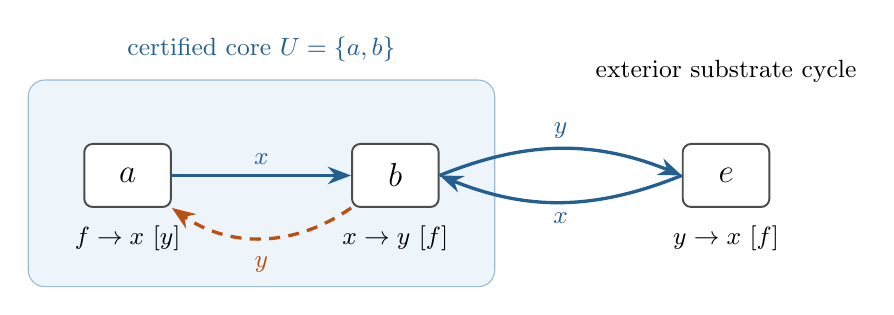
\begin{tikzpicture}[>=Stealth,
  rxn/.style={draw=black!70,rounded corners=3pt,minimum width=11mm,minimum height=8mm,fill=white,line width=.7pt,font=\large},
  sub/.style={->,substrate,line width=1.2pt},
  catl/.style={->,catalytic,line width=1.2pt,dash pattern=on 4pt off 3pt}]
 \node[rxn] (a) at (0,0) {$a$};
 \node[rxn] (b) at (3.4,0) {$b$};
 \node[rxn] (e) at (7.6,0) {$e$};
 \node[below=1mm of a,font=\small] {$f\to x\ [y]$};
 \node[below=1mm of b,font=\small] {$x\to y\ [f]$};
 \node[below=1mm of e,font=\small] {$y\to x\ [f]$};
 \draw[sub] (a) -- node[above,font=\small]{$x$} (b);
 \draw[catl] (b.south west) to[bend left=35] node[below,font=\small,pos=.5,yshift=-1mm]{$y$} (a.south east);
 \draw[sub] (b.east) to[bend left=22] node[above,font=\small]{$y$} (e.west);
 \draw[sub] (e.west) to[bend left=22] node[below,font=\small]{$x$} (b.east);
 \begin{scope}[on background layer]
  \node[fill=corefill,draw=coreedge,rounded corners=6pt,fit=(a)(b),inner xsep=7mm,inner ysep=9mm,yshift=-1mm] (core) {};
 \end{scope}
 \node[above=1mm of core.north,substrate,font=\small] {certified core $U=\{a,b\}$};
 \node[above=6.5mm of e,font=\small] {exterior substrate cycle};
\end{tikzpicture}
\caption{Example~\ref{ex:strict}. Solid blue arrows are substrate-production incidences; the dashed orange arrow is non-food catalytic support. Food catalyses $b$ and $e$. The cycle $b\to e\to b$ in the ambient substrate digraph does not affect the internal rank of $U$.}
\label{fig:strict}
\end{figure}

The example also illustrates why the exterior predicate~\eqref{eq:exterior} must be evaluated through the combined closure: the exterior selection $T=\{e\}$ is not food-generated on its own, yet $\{a,b\}\cup\{e\}\in\FF$. The fibre over $T=\{e\}$ is $\{\{a,b\}\}$ and the fibre over $T=\varnothing$ is $\{\varnothing,\{a,b\}\}$; both satisfy~\eqref{eq:fibre}. An earlier form of Theorem~\ref{thm:main}, which required a rank on the substrate digraph of the whole system, does not apply here, and the formal development records both the certificate of $U$ and the nonexistence of a global rank (Appendix~\ref{app:lean}).

\subsection{A uniform three-chain family}\label{sec:family}

Fix an integer $\ell\ge3$ and let $F=\{f\}$. There are three chains $a_1,\dots,a_\ell$, $b_1,\dots,b_\ell$, $c_1,\dots,c_\ell$ and three gates $g_A,g_B,g_C$. Every chain reaction consumes only $f$. For $j<\ell$ the reaction $a_j$ produces a private molecule $y^A_j$; the last chain reactions and the gates are
\begin{center}
\begin{tabular}{@{}lll@{}}\toprule
Reaction & Transformation & Catalyst\\\midrule
$a_\ell$ & $f\to x_A+u$ & $y^A_{\ell-1}$\\
$b_\ell$ & $f\to u+v$ & $y^B_{\ell-1}$\\
$c_\ell$ & $f\to v+x_C$ & $y^C_{\ell-1}$\\
$g_A$ & $x_A\to z_A$ & $f$\\
$g_B$ & $u+v\to z_B$ & $f$\\
$g_C$ & $x_C\to z_C$ & $f$\\\bottomrule
\end{tabular}
\end{center}
The first chain reaction $a_1$ is catalysed only by the gate product $z_A$, and each $a_j$ with $j\ge2$ is catalysed only by $y^A_{j-1}$; the $B$ and $C$ chains are analogous. The system has $3\ell+3$ reactions and $3\ell+5$ molecules, one food molecule, one catalyst per reaction, at most two reactants and two products per reaction, and its food closure stabilises after two rounds for every selected set.

Let $A$ denote the $A$ chain together with $g_A$, and define $B$ and $C$ similarly. Each is a locally ranked complete-supplier core: $d(a_1)=g_A$, $d(a_j)=a_{j-1}$ for $j\ge2$, and $d(g_A)=a_\ell$, which supplies $x_A$ while food catalyses the gate; the same for $C$; and for $B$, $d(g_B)=b_\ell$ supplies both $u$ and $v$. The only internal substrate incidences are $a_\ell\to g_A$, $b_\ell\to g_B$, $c_\ell\to g_C$, so rank $0$ on chain reactions and $1$ on gates is valid, here even globally.

\begin{proposition}[Exact family]\label{prop:family}
$\FF$ consists exactly of the eight unions of subcollections of $\{A,B,C\}$ together with the $\ell$ sets
\begin{equation}\label{eq:prefix}
 A\cup C\cup\{g_B\}\cup\{b_1,\dots,b_j\},\qquad 0\le j<\ell .
\end{equation}
Consequently
\begin{align}
 M_\ell&=\ell+8,\label{eq:Mell}\\
 f(a_j)=f(c_j)=f(g_A)=f(g_B)=f(g_C)&=\ell+4,\label{eq:freqAC}\\
 f(b_j)&=\ell+4-j\qquad(1\le j\le\ell).\label{eq:freqB}
\end{align}
\end{proposition}
\begin{proof}
Let $W$ be a RAF. Within a chain, the selected reactions form a prefix, because each chain reaction after the first is catalysed only by the product of its predecessor, and a nonempty prefix requires the chain's gate, because the first chain reaction is catalysed only by the gate product. The gate $g_A$ requires $x_A$, produced only by $a_\ell$, so $g_A\in W$ forces all of $A$; likewise for $C$. The gate $g_B$ requires $u$ and $v$: either $b_\ell\in W$, which forces all of $B$, or $a_\ell,c_\ell\in W$, which forces all of $A$ and $C$, and then any proper prefix of the $B$ chain may accompany $g_B$, including the empty prefix. Conversely every set of the stated form is a RAF: all selected chain reactions are food-ready, every selected gate has its substrates from a selected final chain reaction, every gate is food-catalysed, and every selected chain reaction has its catalyst produced by a selected reaction, all within the closure. The $\ell$ sets~\eqref{eq:prefix} are distinct from each other and from the eight whole-core unions, since they contain $g_B$ but not all of $B$; the union with $j=\ell$ is $A\cup B\cup C$.

Every reaction of $A$, of $C$, and every gate lies in four whole-core unions and in all $\ell$ sets~\eqref{eq:prefix}. The reaction $b_j$ lies in the four whole-core unions containing $B$ and in the $\ell-j$ sets~\eqref{eq:prefix} with prefix length at least $j$.
\end{proof}

\begin{corollary}[Sharp average, rare members]\label{cor:sharp}
In the three-chain family the core $B$ has average occupancy exactly one half, while its rarest reaction has occupancy tending to zero and its gate has occupancy tending to one:
\[
 \frac{\sum_{r\in B}f(r)}{|B|\,M_\ell}=\frac12,\qquad
 \frac{f(b_\ell)}{M_\ell}=\frac4{\ell+8}\longrightarrow0,\qquad
 \frac{f(g_B)}{M_\ell}=\frac{\ell+4}{\ell+8}\longrightarrow1 .
\]
Exactly the reactions $b_j$ with $2j\le\ell$ are abundant among the $B$-chain reactions.
\end{corollary}
\begin{proof}
With $|B|=\ell+1$ and~\eqref{eq:freqB}, $\sum_{r\in B}f(r)=(\ell+4)+\sum_{j=1}^{\ell}(\ell+4-j)=\frac{(\ell+1)(\ell+8)}2$. The limits are immediate, and $2(\ell+4-j)\ge\ell+8$ is equivalent to $2j\le\ell$.
\end{proof}

\begin{figure}[htbp]
\centering
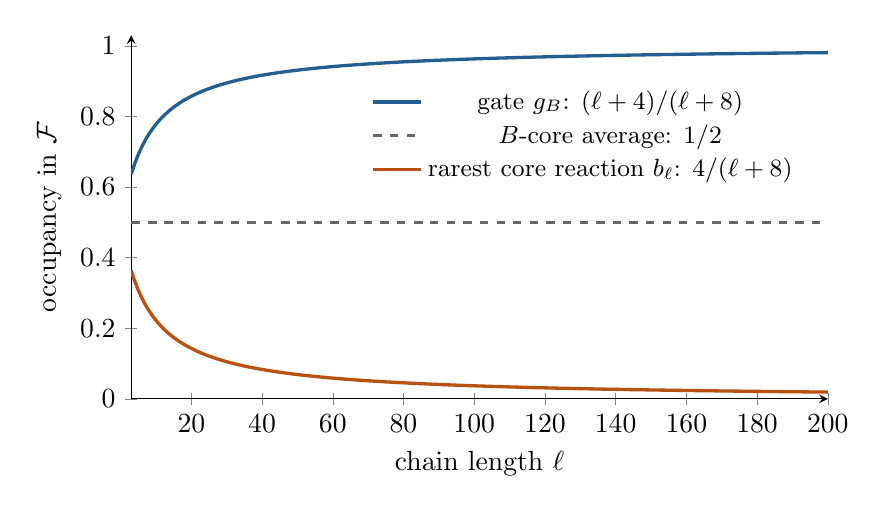
\begin{tikzpicture}
\begin{axis}[width=.86\linewidth,height=6.2cm,xlabel={chain length $\ell$},ylabel={occupancy in $\FF$},
  xmin=3,xmax=200,ymin=0,ymax=1.03,ytick={0,0.2,0.4,0.6,0.8,1.0},
  axis lines=left,grid=none,legend style={draw=none,fill=white,at={(0.97,0.88)},anchor=north east,font=\small},
  every axis plot/.append style={line width=1.2pt},domain=3:200,samples=200]
 \addplot[substrate] {(x+4)/(x+8)};
 \addlegendentry{gate $g_B$: $(\ell+4)/(\ell+8)$}
 \addplot[black!60,dashed] {0.5};
 \addlegendentry{$B$-core average: $1/2$}
 \addplot[catalytic] {4/(x+8)};
 \addlegendentry{rarest core reaction $b_\ell$: $4/(\ell+8)$}
\end{axis}
\end{tikzpicture}
\caption{Occupancies in the three-chain family, from~\eqref{eq:Mell}--\eqref{eq:freqB}. The average over the certified core $B$ equals one half for every $\ell$, while individual core reactions range from almost always present to almost never present. The sharpness concerns the average over a designated core, not the maximum frequency in the whole system: the reactions of $A$ and $C$ have occupancy $(\ell+4)/(\ell+8)$.}
\label{fig:curves}
\end{figure}

The family has several structural properties that place it outside earlier positive results.
\begin{itemize}
\item \emph{No elementary RAF.} Without gates no first chain reaction has a catalyst, so no set of food-ready reactions is a RAF. The elementary-core theorem of~\cite{elementary2026} does not apply; Theorem~\ref{thm:main} applies to each of $A$, $B$ and $C$, and Corollary~\ref{cor:transport}(b) gives three distinct abundant reactions.
\item \emph{Transversal number three.} Every nonempty member of $\FF$ contains a whole core, so the minimum RAF size is $\ell+1$, although only the three gates are not food-ready. The three disjoint cores show that no two reactions meet every nonempty RAF; the three gates do. The two-element transversal argument of~\cite[Lemma~5.6]{elementary2026} therefore does not apply.
\item \emph{Irreducible RAFs do not determine $\FF$.} The only irreducible RAFs are $A$, $B$ and $C$; their unions omit the $\ell$ sets~\eqref{eq:prefix}, which are what make the $B$-chain frequencies nonuniform. A count restricted to unions of irreducible RAFs would report every reaction with frequency $4$ out of $8$.
\item \emph{Not a digraph support family.} Call a family of subsets of a vertex set the support family of a digraph if a set belongs to it exactly when every member has an in-neighbour in the set (loops allowed). $\FF$ is not the support family of any digraph on the $3\ell+3$ reactions: $A$ and $C$ are members, $A\cup\{g_B\}$ and $C\cup\{g_B\}$ are not, but $A\cup C\cup\{g_B\}$ is; a digraph in-neighbour of $g_B$ inside the last set lies in $A$, in $C$, or is $g_B$ itself, and each possibility makes one of the two excluded sets supported. The intrinsic characterisation of digraph support families in~\cite{digraph2026} thus does not cover RAF families with joint reactant requirements.
\end{itemize}

\subsection{Sharpness of the witness fraction}

\begin{example}[All-or-none modules]\label{ex:modules}
For $k\ge1$ take $k$ modules with private molecules $x_i,y_i$ and reactions $p_i:f\to x_i\ [y_i]$, $q_i:x_i\to y_i\ [f]$. Each $\{p_i,q_i\}$ is a locally ranked complete-supplier core ($d(p_i)=q_i$, $d(q_i)=p_i$, $\lambda(p_i)=0$, $\lambda(q_i)=1$), and a set is a RAF exactly when it is a nonempty union of whole modules. Hence $M=2^k$ and $f(r)=2^{k-1}$ for every reaction: the empty-inclusive bound $2f(r)\ge M$ holds with equality for every $r$, and the nonempty-only fraction $2^{k-1}/(2^k-1)$ tends to $1/2$ from above. With $k=1$ this is the two-member family used for the sharpness of Theorem~\ref{thm:distortion}.
\end{example}

The constant $1/2$ in Theorem~\ref{thm:main} therefore cannot be improved, either for the core average (Corollary~\ref{cor:sharp}) or for the best individual witness (Example~\ref{ex:modules}), and the two kinds of sharpness are realised by different mechanisms.

\subsection{The twelve-reaction instance and a conservation lift}\label{sec:twelve}

For $\ell=3$ the family has $M=11$, $N=10$. Figure~\ref{fig:twelve} shows the supplier structure and Table~\ref{tab:frequency} the full frequency table. The proposition proves these values uniformly in $\ell$; an independent exhaustive food-closure computation over all $2^{12}$ subsets confirms them for this instance (Appendix~\ref{app:lean}).

\begin{figure}[htbp]
\centering
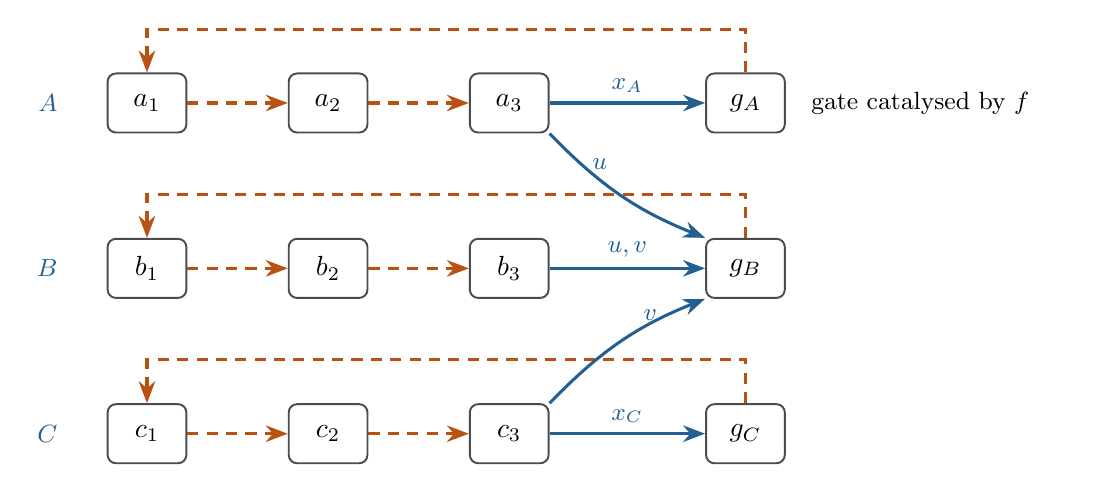
\begin{tikzpicture}[>=Stealth,
  rxn/.style={draw=black!70,rounded corners=3pt,minimum width=10mm,minimum height=7.5mm,fill=white,line width=.7pt},
  sub/.style={->,substrate,line width=1.1pt},
  catl/.style={->,catalytic,line width=1.1pt,dash pattern=on 4pt off 3pt}]
 \foreach \row/\y/\L/\l in {1/4.2/A/a, 2/2.1/B/b, 3/0/C/c}{
   \node[rxn] (\l1) at (0,\y) {$\l_1$};
   \node[rxn] (\l2) at (2.3,\y) {$\l_2$};
   \node[rxn] (\l3) at (4.6,\y) {$\l_3$};
   \node[rxn] (g\L) at (7.6,\y) {$g_{\L}$};
   \draw[catl] (\l1) -- (\l2);
   \draw[catl] (\l2) -- (\l3);
   \draw[catl] (g\L.north) -- ++(0,.55) -| (\l1.north);
 }
 \draw[sub] (a3) -- node[above,font=\small]{$x_A$} (gA);
 \draw[sub] (b3) -- node[above,font=\small]{$u,v$} (gB);
 \draw[sub] (c3) -- node[above,font=\small]{$x_C$} (gC);
 \draw[sub] (a3.south east) to[bend right=12] node[pos=.22,right,font=\small,substrate]{$u$} (gB.north west);
 \draw[sub] (c3.north east) to[bend left=12] node[pos=.8,left,font=\small,substrate]{$v$} (gB.south west);
 \node[right=2mm of gA,font=\small,text width=3.1cm] {gate catalysed by $f$};
 \node[left=5mm of a1,substrate,font=\small] {$A$};
 \node[left=5mm of b1,substrate,font=\small] {$B$};
 \node[left=5mm of c1,substrate,font=\small] {$C$};
\end{tikzpicture}
\caption{The three-chain family at $\ell=3$. Dashed orange arrows are catalytic support along each chain, with the gate product catalysing the first chain reaction. Solid blue arrows supply gate substrates. The cross incidences $a_3\to g_B$ and $c_3\to g_B$ jointly permit the three proper-prefix members~\eqref{eq:prefix}. Every chain reaction consumes only food.}
\label{fig:twelve}
\end{figure}

\begin{table}[htbp]\centering
\caption{Frequencies in the twelve-reaction instance ($\ell=3$, $M=11$). The abundance threshold is $M/2=5.5$; $b_2$ and $b_3$ are rare although they belong to a certified core.}\label{tab:frequency}
\begin{tabular}{@{}lcccc@{}}\toprule
Core & first chain reaction & second & third & gate\\\midrule
$A$ & $f(a_1)=7$ & $f(a_2)=7$ & $f(a_3)=7$ & $f(g_A)=7$\\
$B$ & $f(b_1)=6$ & $f(b_2)=5$ & $f(b_3)=4$ & $f(g_B)=7$\\
$C$ & $f(c_1)=7$ & $f(c_2)=7$ & $f(c_3)=7$ & $f(g_C)=7$\\\bottomrule
\end{tabular}
\end{table}

Deleting one reaction of $B$ gives the following exact panel, by Proposition~\ref{prop:delete}:
\begin{center}
\begin{tabular}{@{}lcc@{}}\toprule
Deleted reaction & RAFs destroyed & nonempty RAFs remaining\\\midrule
$g_B$ & 7 & 3\\ $b_1$ & 6 & 4\\ $b_2$ & 5 & 5\\ $b_3$ & 4 & 6\\\bottomrule
\end{tabular}
\end{center}
The expected number remaining under uniform choice in $B$ is $4.5=(N-1)/2$, attaining~\eqref{eq:expecteddelete}; the individual choices $b_2$ and $b_3$ destroy fewer than half of the RAFs, while $g_B$ and $b_1$ satisfy~\eqref{eq:delete}.

The construction admits a conservation bookkeeping without any change to $\FF$. Assign two units to $f$, one unit to every private chain product and to $x_A,u,v,x_C,z_A,z_C$, and two units to $z_B$. Introduce an inert one-unit molecule $\omega$ and replace every chain reaction $f\to p$ with a single product by $f\to p+\omega$. Then every reaction conserves units: the final chain reactions produce two one-unit molecules from $f$, and the gates $x_A\to z_A$, $u+v\to z_B$, $x_C\to z_C$ balance. Catalysts appear on both sides of a stoichiometric equation and cancel.

\begin{proposition}[Inert-output preservation]\label{prop:waste}
Let $\QQ'$ be obtained from $\QQ$ by adding, to the product sets of some reactions, fresh molecules that are reactants or catalysts of no reaction. Then $\QQ'$ and $\QQ$ have the same RAF family on the same reaction identities.
\end{proposition}
\begin{proof}
Let $X$ be the original molecule set. We show by induction on the stage that $H'_j(W)\cap X=H_j(W)$ for every $W$ and $j$, where $H'$ is the closure in $\QQ'$. The base case is $F$. A reaction is enabled at stage $j$ in $\QQ'$ if and only if its reactants, which lie in $X$, are in $H'_j(W)\cap X=H_j(W)$, so exactly the same reactions fire, and each adds its original products together with inert molecules outside $X$. Hence $H'(W)\cap X=H(W)$. Food generation tests reactants, and catalysis tests catalysts, both subsets of $X$; so every $W$ has the same status in both systems.
\end{proof}

This gives a balanced schematic construction, not a chemical model: it establishes no empirical catalysts, thermodynamic feasibility, flux or persistence, and a biochemical reconstruction would have to supply those ingredients separately.

\section{Certificates and computation}\label{sec:algorithms}

A certificate for Theorem~\ref{thm:main} consists of a nonempty candidate $U$, a rank $\lambda$ on $U$ and a supplier $d(r)\in U$ for each $r\in U$. Validation checks~\eqref{eq:supplier} for each pair $(d(r),r)$ and~\eqref{eq:rank} for every internal incidence, including self-incidences. Nothing outside $U$ is read, no RAF is enumerated, and no closure is computed: the theorem supplies RAF status and abundance. In particular the validation cost is independent of the size of the exterior.

With $k=|U|$ and molecules encoded as bitsets of $m$ coordinates and word size $w$, constructing the internal substrate digraph costs $O(k^2\lceil m/w\rceil)$ word operations and a topological sort costs $O(k+e)$ for $e$ internal edges, which also produces a rank if one exists. Checking the supplied suppliers costs $O(k\lceil m/w\rceil)$; searching for suppliers among all internal pairs, when none are supplied, has the same quadratic bound as the graph construction. Input parsing is additional. With set-based representations the same bounds hold in units of set intersection and subset tests.

Three capabilities must be kept apart. \emph{Validation} checks a supplied candidate, as above. \emph{Discovery} proposes candidates; a directed cycle in the complete-supplier digraph, with edges $p\Rightarrow r$ whenever $p$ is a complete supplier of $r$, is a natural candidate, but any nonempty internally ranked, internally supplied set is admissible, and the theorem does not claim polynomial-time complete discovery of all certifiable cores. \emph{Witness identification} chooses an individually abundant reaction inside $U$; the certificate does not compute frequencies, and Table~\ref{tab:frequency} shows that a certified core can contain rare reactions. A failed candidate means only that this certificate failed, not that no RAF or no abundant reaction exists. The accompanying implementation~\cite{repository2026} validates a supplied core locally, accepts Example~\ref{ex:strict} although the global-rank test rejects it, and rejects a missing supplier and an internal self-loop; individual frequencies in its worked output come from a separately labelled exhaustive check.

\section{Scope and open problems}\label{sec:scope}

The results are statements about finite set families. They assert nothing about concentrations, fluxes, persistence under dynamics, thermodynamic feasibility or the chemical realisability of the molecules in the examples, and a reaction that lies in half of all RAFs is not thereby essential to any of them. The weighted results allow arbitrary nonnegative weights on exterior contexts, and weights on individual members with bounded within-fibre distortion; arbitrary weights on individual RAFs are outside the theorem.

The sufficient condition proved here is the existence of a locally ranked complete-supplier core. It contains the elementary cores of~\cite{elementary2026}, whose universal construction shows that no condition satisfied by the producer--gate source can be sufficient short of the full conjecture. Between the two lie the following questions.

\begin{question}
The rank condition~\eqref{eq:rank} is needed in some form (Remark~\ref{rem:excludes}), but it excludes cores in which a non-food reactant is produced by its own consumer. Is there a seeded variant, requiring for instance that every internal substrate cycle contain a reaction whose reactants are available from outside the cycle, under which Lemma~\ref{lem:adapter} survives?
\end{question}

\begin{question}
The single-supplier condition asks one reaction to meet all requirements of $r$. The universal construction shows that fully independent suppliers cannot be allowed. Is there an intermediate condition, for instance two suppliers with a common coordinate in every failing configuration, under which an injection with the collision structure of Lemma~\ref{lem:count} still exists?
\end{question}

\begin{question}
The three-chain family and its relatives have exactly three non-food-ready reactions, each a gate of a core. Does every system with a RAF and exactly three non-food-ready reactions have an abundant reaction? The transversal argument of~\cite{elementary2026} stops at two, and the family shows that the three gates can all be non-rare while the cores contain rare reactions.
\end{question}

\begin{question}
Which certified cores admit a witness that is stable across a specified family of exterior contexts, or an individually abundant reaction identifiable from the certificate alone? Corollary~\ref{cor:sharp} shows that the gate of a chain core is asymptotically the right choice in the three-chain family; whether a general rule exists is open.
\end{question}

The strongest positive statement known for general RAF families remains the constant of the entropy method~\cite{gilmer2022constant,alweiss2022improved,chase2022approximate,sawin2022improved,cambie2022better}, a reaction in a $0.38$ fraction of all RAFs of any system with a RAF. Whether the RAF structure can push that constant to $1/2$ is, by the equivalence theorem of~\cite{elementary2026}, exactly the union-closed sets conjecture.

\appendix

\section{Formal verification}\label{app:lean}

\subsection{Environment and receipts}

The formal development is written in Lean~4 (toolchain \lean{leanprover/lean4:v4.30.0}) against Mathlib at commit \lean{c5ea0035} (the \lean{v4.30.0} tag), in the directory \lean{proofs/RAF/Frankl/} of the companion repository~\cite{repository2026}. The public entry module \lean{LocalSupplierPaper.lean} imports the four result modules. It was compiled with \lean{-DwarningAsError=true}; the compiler produced no output. The verification receipt records the SHA-256 of the root source, of the $26$ local dependency sources and of the Lake manifest, together with an elaboration probe of each exported declaration; every exported theorem depends only on \lean{Classical.choice}, \lean{Quot.sound} and \lean{propext}, with no \lean{sorry} and no \lean{native_decide}. The receipt used here is:

\begin{center}\small
\begin{tabular}{@{}llll@{}}\toprule
Root module & Declarations & Root SHA-256 (prefix) & Elaboration time\\\midrule
\lean{RAF/Frankl/LocalSupplierPaper.lean} & 7 & \lean{5216507abc656138} & 154.4\,s\\\bottomrule
\end{tabular}
\end{center}

The earlier global-rank form of the theorem, exported as \lean{abundance_beyond_elementary} from the module \lean{SupplierCycleCertificate}, is retained unchanged with its own receipt; Example~\ref{ex:strict} separates the two.

The RAF semantics is defined literally as in Definition~\ref{def:crs}: a structure \texttt{CRS M R} with \lean{food}, \lean{inputs} and \lean{outputs}, a relation \texttt{Catalysis M R}, the stage closure \texttt{closureAt Q S k}, the predicates \lean{FoodGenerated}, \lean{CatalyzedFromClosure} and \lean{IsRAF}, and the finite families \lean{rafFamily} (nonempty RAFs) and \lean{fixedFamily} (the family $\FF$). The hypotheses of Definition~\ref{def:core} are \lean{CompleteSupplier}, \lean{SupplierCore} and \lean{InternalSubstrateRank}; the exterior fibre~\eqref{eq:fibredef} is \lean{extensionFibre}, and the local predicate~\eqref{eq:local} is \lean{LocalSupply}.

\subsection{Correspondence}

\begin{center}\small
\renewcommand{\arraystretch}{1.12}
\begin{tabular}{@{}>{\raggedright\arraybackslash}p{.34\linewidth}>{\raggedright\arraybackslash}p{.61\linewidth}@{}}\toprule
Article statement & Lean declaration (namespace \lean{RAF.Frankl}) and module\\\midrule
Lemma~\ref{lem:adapter}, rank induction & \lean{internal_rank_foodGenerated} (\lean{LocalRankedClosure})\\
Lemma~\ref{lem:adapter}, equivalence~\eqref{eq:adapter} & \lean{local_rank_fibre_iff}; monotonicity of~\eqref{eq:exterior} is \lean{closureExterior_mono}\\
Lemma~\ref{lem:count} & \lean{CommonSupplier.supported_upward_average} (\lean{CommonSupplierConditioning}); the injection is \lean{conditionedCellMap}\\
Theorem~\ref{thm:main}, all four conclusions & \lean{locally_ranked_supplier_abundance} (\lean{LocallyRankedSupplierCore}); components \lean{local_supplierCore_isRAF}, \lean{localSupplierFibre_average}, \lean{local_supplier_core_global_average}, \lean{local_supplier_core_exists_abundant}\\
Corollary~\ref{cor:transport}(a), food enlargement and catalysis enlargement with fixed core incidences & \lean{local_certificate_transport} (\lean{LocalSupplierEmbedding})\\
Corollary~\ref{cor:transport}(b) & \lean{disjoint_local_cores_witnesses}\\
Corollary~\ref{cor:weights} (unnormalised) & \lean{local_supplier_exterior_weights} (\lean{LocalSupplierWeights})\\
Theorem~\ref{thm:distortion}, inequalities~\eqref{eq:distortion} (unnormalised) & \lean{local_supplier_bounded_weights}; the fibre aggregation is \lean{weighted_fibre_aggregation} (\lean{SupplierWeightedCounting})\\
Proposition~\ref{prop:delete}, bound~\eqref{eq:delete} as a count of original RAFs omitting $r$ & \lean{local_supplier_deletion} (\lean{SupplierDeletion}); the partition $N=N_\after+f(r)$ is \lean{deletion_partition}\\
Example~\ref{ex:strict}, family~\eqref{eq:strict} & \lean{LocalSupplierExample.exact_fixed_family} (\lean{LocalSupplierExamples}); also \lean{certified}, \lean{no_global_rank}, \lean{exterior_not_generated}\\\bottomrule
\end{tabular}
\end{center}

\subsection{What is and is not formalised}

The formal statements are literal. \lean{locally_ranked_supplier_abundance} takes an arbitrary \lean{CRS}, an arbitrary catalysis relation, a finite set \lean{U}, a rank function with \lean{InternalSubstrateRank}, and \lean{SupplierCore}, and returns the conjunction of \texttt{IsRAF Q C U}, the fibre inequality~\eqref{eq:fibre} for every \lean{T}, the global inequality~\eqref{eq:global} and the witness~\eqref{eq:witness}, all for the full system; no projection, feedback or average hypothesis appears. The weighted exports are the unnormalised inequalities $|U|\sum_Ww(W)\le(1+\kappa)\sum_Ww(W)|W\cap U|$ and their witnesses, over real weights bounded fibrewise by $b_T\le w\le\kappa b_T$; division by the positive total mass, which gives the probability statements of Section~\ref{sec:consequences}, is ordinary arithmetic. The deletion export counts original RAFs omitting $r$; the identification of these with the RAFs of the reduced system, and the expectation bound, are proved in Proposition~\ref{prop:delete}. The transport export covers enlargement of food and of the catalysis relation on a fixed reaction type with unchanged core incidences; addition and deletion of exterior reactions, which change the reaction type, are covered by the ordinary argument of Corollary~\ref{cor:transport}. Proposition~\ref{prop:elementary}, Remark~\ref{rem:excludes}, Proposition~\ref{prop:family}, Corollary~\ref{cor:sharp}, Example~\ref{ex:modules}, the structural properties of the three-chain family and Proposition~\ref{prop:waste} have ordinary proofs above and are not claimed as separately kernel-verified parametric constructions. The finite data of Section~\ref{sec:twelve} (the family for $\ell=3$, the frequencies, the deletion panel, the unit balance of the lifted system and the identity of its family) are replayed by an independent exhaustive script in the paper's source folder, which also checks Proposition~\ref{prop:family} for $3\le\ell\le7$ and Example~\ref{ex:modules} for $k\le5$; that script is a diagnostic, not a proof substitute.

\subsection{Reproduction}

From the repository root, with the pinned toolchain, the strict verification of the entry module is
\begin{quote}\small\ttfamily
python scripts/verify\_proof.py proofs/RAF/Frankl/LocalSupplierPaper.lean\\
\ \ --declaration RAF.Frankl.locally\_ranked\_supplier\_abundance\\
\ \ --declaration RAF.Frankl.local\_supplier\_bounded\_weights\\
\ \ --declaration RAF.Frankl.local\_supplier\_exterior\_weights\\
\ \ --declaration RAF.Frankl.LocalSupplierExample.exact\_fixed\_family\\
\ \ --declaration RAF.Frankl.local\_supplier\_deletion\\
\ \ --declaration RAF.Frankl.disjoint\_local\_cores\_witnesses\\
\ \ --declaration RAF.Frankl.local\_certificate\_transport\\
\ \ --timeout 360 --output LocalSupplierPaper.verify.json
\end{quote}
The bridge fixes the frozen Mathlib working directory, treats warnings as errors and records the source hashes and the axioms of each declaration.

\section*{Acknowledgements}
To be inserted.

\bibliographystyle{plainnat}
\bibliography{refs}

\end{document}
